\section{مقدمه}


به طور معمول، هنگامی که یک مدل یادگیری ماشین را آموزش می‌دهیم به یک مجموعه از داده‌های آموزش\LTRfootnote{training set} دسترسی داریم که به کمک آن می‌توانیم میزان خطا را بر روی این داده‌ها محاسبه کنیم. 
به این خطا، خطای یادگیری\LTRfootnote{training error} گفته می‌شود و ما به دنبال کاهش این خطا هستیم. 

تا به اینجای کار یک مسئله‌ بهینه‌سازی را تعریف کرده‌ایم. آنچه یادگیری ماشین را نسبت به بهینه‌سازی\LTRfootnote{optimization} متمایز می‌کند آن است که در یادگیری ماشین ما می‌خواهیم که خطای تعمیم\LTRfootnote{generalization error} یا خطای آزمون\LTRfootnote{test error} نیز کاهش پیدا کند.
خطای تعمیم را به صورت میزان خطای مورد انتظار بر روی داده‌های دیده‌ نشده تعریف می‌کنیم.
برای تخمین خطای تعمیم یک مدل یادگیری ماشین، می‌توانیم میزان خطای این مدل را بر روی یک مجموعه از داده‌های آزمون\LTRfootnote{test set} محاسبه کنیم که مستقل از داده‌های آموزش باشد.

حال این پرسش مطرح می‌شود که چگونه می‌توانیم میزان خطای مدل را بر روی داده‌های آزمون کاهش دهیم در صورتی که تنها به داده‌های آموزش دسترسی داریم؟
بر اساس نظریه یادگیری آماری\LTRfootnote{statistical learning theory} می‌توانیم به این پرسش پاسخ دهیم. اگر داده‌های آموزش و آزمون به صورت کاملاً دلخواهانه انتخاب شده باشند، و فرض خاصی بر روی داده‌ها نداشته باشیم، نمی‌توانیم کار زیادی انجام دهیم. 
اگر بتوانیم نسبت به نحوه‌ی جمع‌آوری داده‌های آموزش و آزمون فرضیاتی داشته باشیم، می‌توانیم کمی پیشروی کنیم. فرض می‌کنیم داده‌های آموزش و آزمون با استفاده از یک توزیع احتمالاتی مشترک تحت فرآیندی به نام فرآیند تولید داده\LTRfootnote{data-generating process} ایجاد شده باشند و هر یک از نمونه‌های جمع‌آوری شده مستقل از سایر نمونه‌ها باشد.\LTRfootnote{independent and identically distributed (i.i.d.) assumptions}
با کمک این فرض می‌توانیم در یک چارچوب احتمالاتی به مطالعه‌ رابطه میان خطای یادگیری و خطای آزمون بپردازیم.

در فرآیند‌های یادگیری ماشین ما ابتدا یک نمونه‌برداری انجام می‌دهیم تا مجموعه‌ داده‌های یادگیری بسازیم، سپس با استفاده از الگوریتم‌های یادگیری ماشین تلاش می‌کنیم تا خطای آموزش را کاهش دهیم. در این صورت اتنظار می‌رود که مقدار خطای آزمون بزرگ‌تر یا مساوی با مقدار خطای آموزش باشد. در این صورت می‌توانیم عوامل مؤثر در عملکرد الگوریتم‌های یادگیری ماشین را به صورت زیر خلاصه کنیم:
\begin{enumerate}
    \item کاهش خطای آموزش
    \item کاهش اختلاف خطای‌ آموزش و خطای آزمون
\end{enumerate}
هر یک از این دو عامل، به چالش‌های بنیادینی که در یادگیری ماشین با آن‌ها مواجه هستیم، یعنی کم‌برازش\LTRfootnote{underfitting} و بیش‌برازش\LTRfootnote{overfitting}، اشاره می‌کنند که در ادامه به معرفی آن‌ها می‌پردازیم. 

% Underfitting
\subsection{کم‌برازش}

کم‌برازش  هنگامی رخ می‌دهد که نمی‌توانیم مقدار خطای مدل را بر روی داده‌های یادگیری کاهش دهیم. در این صورت خطای آموزش نسبتاً مقداری بزرگ خواهد داشت. با توجه به فرض‌هایی که در مورد داده‌ها داشتیم، انتظار می‌رود که مقدار خطای آزمون نیز نسبتاً بزرگ باشد.

% Overfitting
\subsection{بیش‌برازش}

بیش‌برازش هنگامی رخ می‌دهد که مدل آموزش داده شده عملکرد مناسبی در برابر داده‌های یادگیری داشته باشد، ولی در برابر داده‌های دیده نشده قادر به تعمیم نباشد و عملکرد نامناسبی از خود نشان دهد. در این صورت می‌توان گفت که خطای آموزش مدل نسبتاً کوچک است ولی خطای آزمون آن نسبتاً بزرگ است. به بیانی دیگر خطای آموزش و خطای آزمون اختلاف نسبتاً بزرگی دارند.

% Capacity
\subsection{ظرفیت*}

‌می‌توانیم احتمال بیش‌برازش یا کم‌برازش یک مدل را توسط ظرفیت\LTRfootnote{capacity} آن کنترل کنیم. به زبان ساده ظرفیت یک مدل بیانگر قابلیت برازش گستره‌ای از توابع مختلف توسط مدل است. مدل‌هایی که ظرفیت بالایی دارند می‌توانند با حفظ خواص حاضر در مجموعه داده‌های آموزش دچار بیش‌برازش شوند و عملکرد مناسبی بر روی داده‌های تست نداشته باشند.

یک روش برای کنترل ظرفیت یک الگوریتم یادگیری، انتخاب فضای فرضیه‌\LTRfootnote{hypothesis space} آن است. فضای فرضیه یک الگوریتم یادگیری، مجموعه توابعی است که مدل مجاز به گزینش آن‌ها به عنوان پاسخ مسئله است.

برای مثال فضای فرضیه الگوریتم رگرسیون خطی\LTRfootnote{linear regression} شامل تمامی توابع خطی ورودی‌های آن می‌باشد. ما می‌توانیم این الگوریتم را به گونه‌ای تعمیم دهیم (با افزودن درجات بالاتر ورودی‌ها به مجموعه‌ داده‌های آموزش) که فضای فرضیه‌ آن علاوه بر توابع خطی، توابع چندجمله‌ای را نیز در برگیرد. با انجام این کار ظرفیت مدل افزایش می‌یابد. برای نمونه شکل \ref{fig:Capacity} را در نظر بگیرید.
\begin{figure}
    \centering
    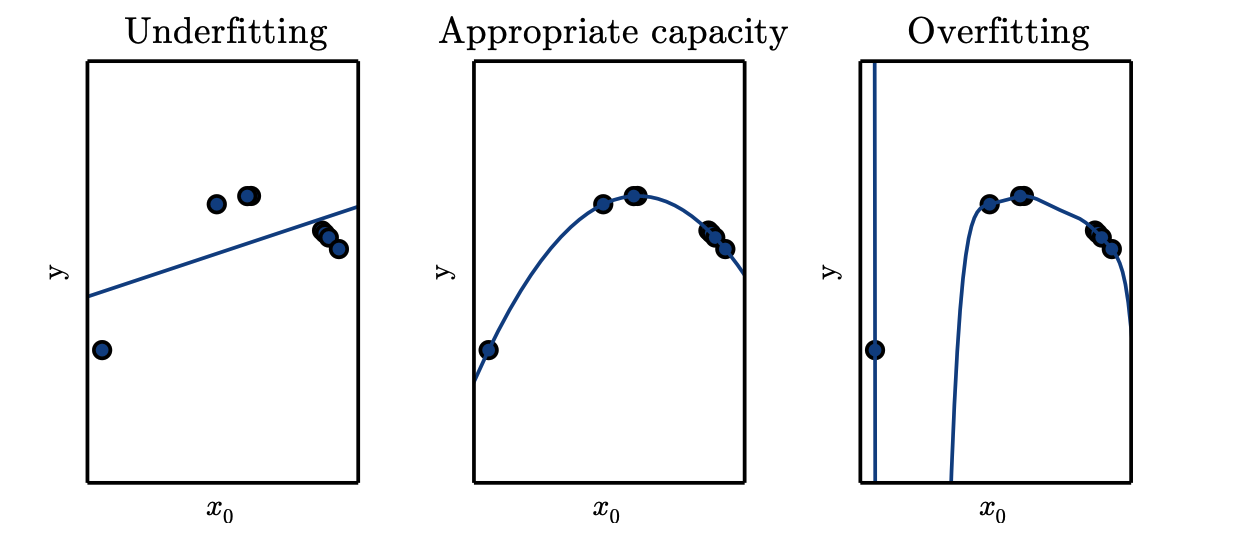
\includegraphics[width=\textwidth]{figs/Capacity.png}
    \caption{در تصویر فوق ۳ مدل را بر روی یک مجموعه از داده‌ها آموزش می‌دهیم. داده‌های فوق با یک نمونه‌ برداری تصادفی از مقادیر $x$ و محاسبه مقادیر $y$ توسط یک تابع درجه دو بدست‌ آمده‌اند. 
    (چپ)
    یک مدل خطی آموزش‌ داده شده بر روی داده‌های فوق، از کم‌برازش رنج می برد و نمی‌تواند انحنای موجود در
    داده‌ها را ثبت کند.
    (وسط)
    یک مدل درجه دوم آموزش داده شده بر روی داده‌های فوق، به خوبی به نقاط دیده نشده تعمیم می‌یابد و از مقدار قابل توجهی کم‌برازش یا بیش‌برازش رنج نمی‌برد.
    (راست)
    یک مدل چندجمله‌ای از درجه ۹ آموزش داده شده بر روی داده‌های فوق، از بیش‌برازش رنج می‌برد ولی اگرچه مدل آموزش داده شده از همه‌ی نقاط به صورت دقیق عبور می‌کند، قادر به تعمیم بر روی داده‌های دیده نشده نیست.}
    \label{fig:Capacity}
\end{figure}

تا به اینجای کار تنها با روش تغییر تعداد ویژگی‌ها\LTRfootnote{feature} و افزودن پارامتر‌های جدید متناظر با این ویژگی‌ها ظرفیت مدل را تغییر دادیم. اما روش‌های دیگری برای تغییر ظرفیت یک مدل نیز وجود دارد. به همین منظور به سراغ مفهومی به نام ظرفیت توصیفی\LTRfootnote{representational capacity} می‌رویم. در واقع هنگامی که یک مدل را برای آموزش بر می‌گزینیم، در اصل خانواده‌ای از توابعی که الگوریتم یادگیری می‌تواند آن‌ها را انتخاب کند تا خطا را کاهش دهد مشخص می‌شود. در عمل الگوریتم‌های یادگیری اغلب قادر نخواهند بود که بهترین تابع را پیدا کنند بلکه صرفاً قادر به یافتن توابعی هستند که مقدار خطای آموزش را به اندازه قابل توجهی کاهش دهند. بی‌نقص نبودن فرآیند بهینه‌سازی باعث می‌شود که ظرفیت مؤثر\LTRfootnote{effective capacity} یک مدل کمتر از ظرفیت توصیفی آن باشد.